Google Glass, or simply ``Glass'' as the device is known within Google, is a head mounted display (HMD) that can be seen as an augmented reality device\footnote{See section \ref{subsubsec:augmentedrealityvsvirtualreality}} designed to bring notifications to the user more easily than a smartphone does. According to Google ``Glass is designed to be there when the user needs it and to stay out of the way when the user does not''.\cite{glassDesignPrinciples} Google Glass is meant to give the user relevant information at relevant times.\\ 
%\url{https://developers.google.com/glass/design/principles}

	\begin{figure}[ht!]
		\centering
		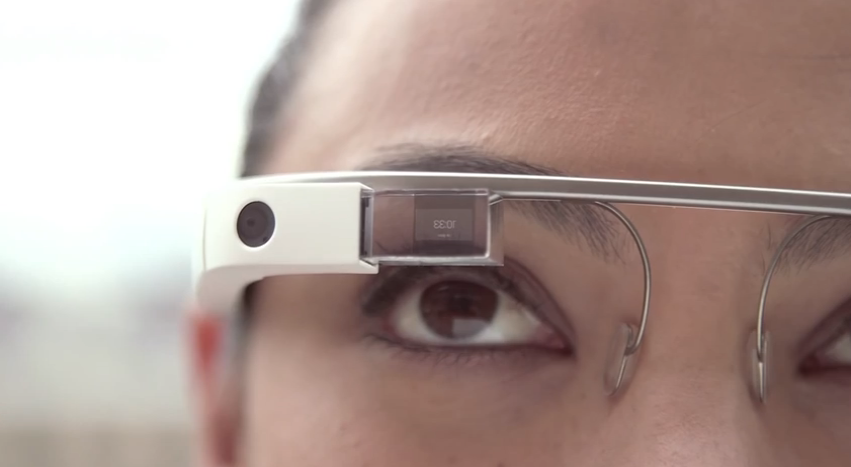
\includegraphics[width=110mm]{images/GoogleGlassHardware}
		\caption{Google Glass is a small head mounted display equipped with a touchpad, a camera and a microphone.\cite{ImagesGoogleGlassUI}}
		\label{GoogleGlassUI}
	\end{figure}

Google Glass is partially controlled with a touchpad (Google Glass can also be controlled with voice command). The touchpad sits on the right hand side of the user's glass frame and runs from the temple to the ear. When the user touches anywhere on the touchpad Google Glass ``wakes up'' from stand by and displays the start screen (which consists of a clock). The display is mounted above the user's line of sight, on the right hand side. The display can be slightly adjusted so that the user can see everything displayed. \\








%	\begin{figure}[ht!]
%		\centering
%		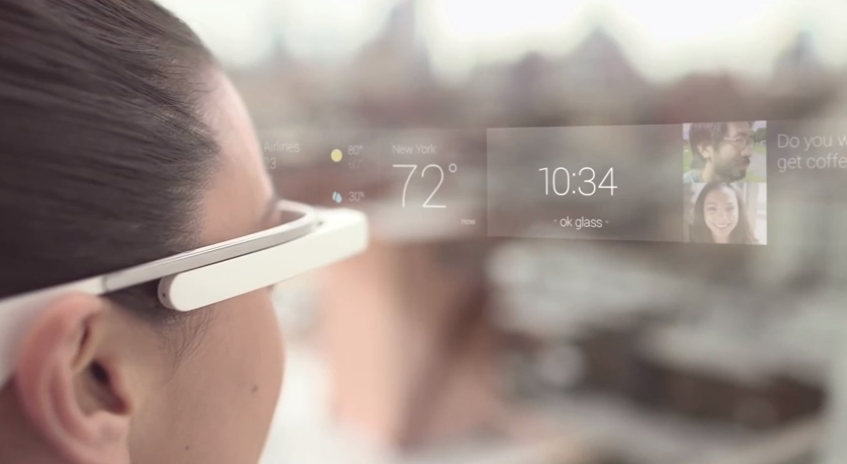
\includegraphics[width=110mm]{images/GoogleGlassUI}
%		\caption{A virtual representation of the Google Glass user interface as the graphical user interface is perceived by the user.\cite{ImagesGoogleGlassUI}}
%		\label{GoogleGlassUI}
%	\end{figure}
	
	
	




%The graphical user interface (GUI) is called a timeline (see Figure \ref{GoogleGlassUI}). The timeline consists of a row of cards. Cards are basic applications such as a clock or information about the weather. Cards can also represent more in-depth applications, on Google Glass called ``Immersions''. An immersion handles activities such as browsing an image gallery or playing a game.\\

%On the timeline cards to the left of the home screen are upcoming activities such as an event in the user's calendar or an upcoming flight. Cards to the right of the home screen are from the past. Cards from the past will for instance show text messages or photos. When the user wants to turn of Google Glass the user swipes down on the touchpad. Swiping down on the touchpad will put Google Glass in stand by. If the user wants to turn of Google Glass entirely there is a power button on the opposite side of the touchpad. Holding down the power button for a few seconds will turn of Google Glass. For a better visual understanding of how Google Glass works see Figure \ref{GoogleGlassUI} as well as the video referenced in the caption.\\

%Glass uses a small display placed to the upper right of the user's line of sight and is mounted on the user as a regular pair of glasses. Equipped with a camera, microphone and speakers it is capable of performing a lot of the tasks users normally would do on a smartphone such as taking photographs, video chatting, writing text messages.


\subsubsection{Augmented Reality vs Virtual Reality}
\label{subsubsec:augmentedrealityvsvirtualreality}

[TODO WRITE ABOUT HUD AND HMD]

When discussing head mounted displays it is possible that the first image that pops into ones head is similar to Figure \ref{OculusRift}. What is important to note about Oculus Rift (Figure \ref{OculusRift}) and other similar product that completely covers the user's eyes is that these are all virtual reality devices. Virtual reality is not the same as augmented reality, which is what Google Glass gives the user.



	\begin{figure}[ht!]
		\centering
		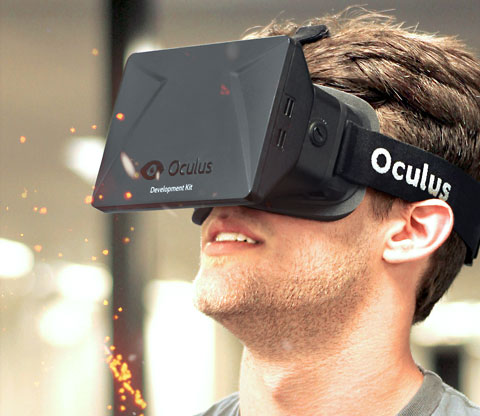
\includegraphics[width=110mm]{images/OculusRift}
		\caption{The virtual reality device Oculus Rift is a head mounted display that covers the user's eyes completely\cite{ImagesOculusRift}}
		\label{OculusRift}
	\end{figure}





The difference lies in how much of what the user can see is computer generated. In a virtual reality the entire environment is computer generated. Augmented reality on the other hand is based in reality where computer generated elements of the environment help enhance reality. In other words: virtual reality replaces reality and augmented reality enhance reality. Since Google Glass does not remove the user from reality but rather display information that can be consumed at the same time as the user experience the real world Google Glass is an augmented reality device compared to Oculus Rift which is a virtual reality device.

TODO --- ADD HUD vs AUGMENTED REALITY!!!!!!


%What is it?
%Augmented Reality vs Virtual Reality
%Define Augmented Reality
%Define Virtual Reality
